
\textbf{Remarque préliminaire}

Pour préciser les types des arguments et du résultat d'une fonction à écrire, on utilisera l'écriture suivante : 
\pyv{def maFonction(n:int, x:float) -> str :}. \pyv{maFonction} est une fonction prenant deux arguments, \pyv{n} de type \pyv{int} et \pyv{n} de type \pyv{int}, et renvoyant un objet de type \pyv{str}.


\exo{Décryptage de texte}



\setcounter{section}{1}

\subsection{Indication sur les méthodes associées aux chaînes de caractères}

Les attributs suivants s'appliquent à des variables de type de chaîne de caractère :
\begin{itemize}
\item \pyv{.isalpha} renvoie \pyv{True} si c'est une des 26 lettres de l'alphabet et \pyv{False} sinon.
\begin{pyconsole}
'c'.isalpha()
'1'.isalpha()
\end{pyconsole}
\item \pyv{.index(x)} renvoie l'indice de la première occurrence de \pyv{x} :
\begin{pyconsole}
'hello'.index('l')
\end{pyconsole}
\item \pyv{.count(x)} renvoie le nombre d'occurrences de \pyv{x} :
\begin{pyconsole}
'hello'.count('l')
\end{pyconsole}
\end{itemize}

\subsection{Le chiffrement de César}



Le \textbf{chiffrement de César} est un des tout premier code de chiffrement qui ait existé. 

La méthode est simple : il suffit de décaler toutes les lettres de l'alphabet du même nombre de lettres. 



Par exemple en choisissant un décalage de 3, le A devient le D, le B devient le E, le C devient le F et ainsi de suite. Pour la fin de l'alphabet, il suffit de revenir au début : le W devient Z, le X devient A, le Y devient B et le Z devient C. Ainsi un message comme << la metamorphose >> devient par décalage d'une lettre << mb nfubnpsqiptf >>, ce qui est incompréhensible pour le non initié.


\question{Avec des instructions python, définir trois chaînes de caractères nommées \textit{alphabet}, \textit{mess} et \textit{code} contenant respectivement les caractères de l'alphabet, un message à chiffrer (exemple << la metamorphose >>) et le message crypté (vide initialement). On se limitera à des lettres minuscules non accentuées. Les autres caractères (espaces, chiffres...) seront gardés tels quels (non chiffrés).}



\question{Comment est codé le message << franz >> avec une valeur de décalage $n=3$ ?}

\question{Écrire une fonction \pyv{def decalage(c:str, n:int) -> str:} permettant de renvoyer un caractère chiffré avec le chiffrement de César.}

%\question{En utilisant les fonctionnalités découvertes dans la première partie, établir un algorithme permettant de chiffrer un message par le code de César, pour un décalage $n$ donné. La fonction aura la signature suivante :
%\pyv{def chiffrement_cesar(mess:str, n:int) -> str:}. }

\question{Etablir un algorithme permettant de chiffrer un message par le code de César, pour un décalage $n$ donné. La fonction associée à cet algorithme aura la signature suivante :

\pyv{def chiffrement_cesar(mess:str, n:int) -> str:}. }




\question{Proposer ensuite l'algorithme de déchiffrement qui affiche le message chiffré en clair, en supposant que $n$ est inconnu. L'utilisateur choisira parmi les déchiffrements proposés celui qui a du sens ! La fonction aura la signature suivante :
\pyv{def decryptage_cesar(code:str) -> None:}.}


%
%\question{Pouvez-vous déchiffrer ce message secret intercepté dans un couloir du lycée : {\em << xq bdaotmuz pqhaud eqdm gz egvqf pq yapqxuemfuaz >>}. Quelle est la faiblesse de ce type de code ?}

\question{Quelle est la faiblesse de ce type de code ? Proposer en deux lignes une méthode permettant de déterminer (casser) la clé.} 



\subsection{Le chiffre de Vigenère}

\begin{figure}[!htb]
\begin{minipage}{0.5\textwidth}
On étudie maintenant la méthode de chiffrement de Vigenère. Pour comprendre le système de chiffrement, on commence par créer la table  Vigenère : on recopie $26$ fois l'alphabet en ligne et à chaque saut de ligne on décale d'une lettre vers la droite comme sur la figure \ref{fig:vigenere}.

Cet algorithme fonctionne à l'aide d'une clé de chiffrement : une chaîne de caractère (typiquement un mot).

Prenons un exemple, mettons que l'on veuille coder \og anticonstitutionnellement\fg~avec la clé \og roue\fg~. Pour ce faire, on crée le tableau présenté table \ref{TabVig} dont la première ligne contient le message à coder, et la deuxième la clé répétée autant de fois que nécessaire pour atteindre la longueur du texte à coder. On fait alors une lecture colonne par colonne de ce tableau et dans chaque colonne :
\begin{enumerate}
\item la première ligne donne l'abscisse dans la table de la lettre à coder;
\item la deuxième donne l'ordonnée dans la table de la lettre à coder;
\end{enumerate}
Ainsi le chiffrement du mot \og anticonstitutionnellement\fg~ avec la clé \og roue\fg~ est obtenue dans la table \ref{TabVig}.
\end{minipage}
\begin{minipage}{0.5\textwidth}
	\centering
		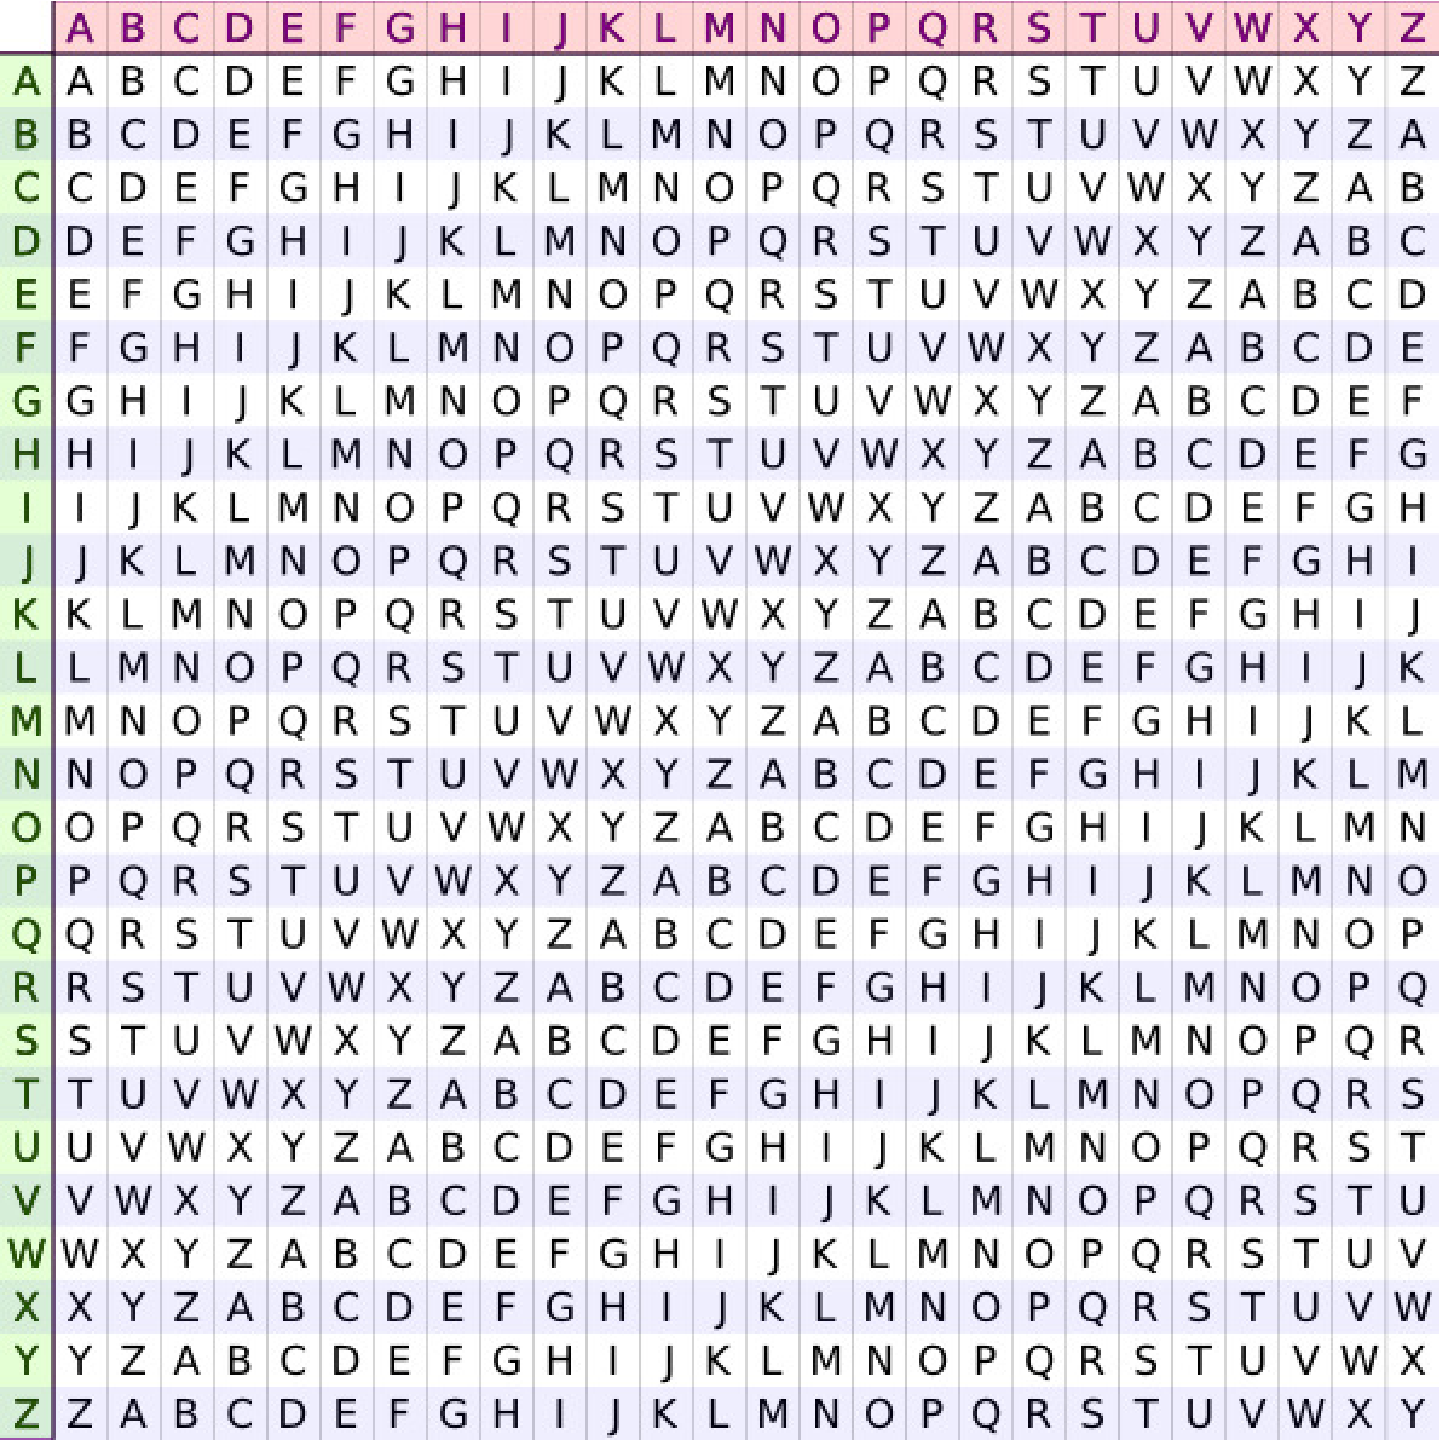
\includegraphics[width=0.95\textwidth]{vigenere.pdf}
	\caption{Table de Vigenère}
	\label{fig:vigenere}
\end{minipage}
\end{figure}




\begin{table}[htbp]
	\centering
		\begin{tabular}{|l|*{25}{|c}|}
		\hline
			mot & a & n & t & i & c & o & n & s & t & i & t & u & t & i & o & n & n & e & l & l & e & m & e & n & t \\
			\hline
			clé & r & o & u & e & r & o & u & e & r & o & u & e & r & o & u & e & r & o & u & e & r & o & u & e & r \\
			\hline
			code & r & b & n & m & t & c & h & w & k & w & n & y & k & w & i & r & e & s & f & p & v & a & y & r & k \\
			\hline
		\end{tabular}
		\caption{Exemple de chiffrement de Vigenère}
		\label{TabVig}
\end{table}


La méthode de chiffrement par lecture de la table est une méthode adaptée \og aux humains\fg, ainsi on réfléchira à l'implémentation d'un algorithme plus efficace en s'aidant de l'exemple.

On dispose de la variable \pyv{alphabet= "abcdefghijklmnopqrstuvwxyz"}. 

On donne le bloc d'instruction suivant : 

\begin{pyverbatim}
alphabet= "abcdefghijklmnopqrstuvwxyz"
for i in range(26):
    alphabet = alphabet[1:]+alphabet[:1]
    print (alphabet)
\end{pyverbatim}

\question{Combien de lignes seront affichées ? Quelles seront les deux premières lignes affichées  ?}

\question{Écrire la fonction \pyv{def generer_table()->list :} qui retourne la table de Vigenère sous la forme d'une liste de listes.}
Le résultat sera de la forme suivante :
\footnotesize{
\begin{pyverbatim}
[['a','b','c','d','e','f','g','h','i','j','k','l','m','n','o','p','q','r','s','t','u','v','w','x','y','z'], 
 ['b','c','d','e','f','g','h','i','j','k','l','m','n','o','p','q','r','s','t','u','v','w','x','y','z','a'],
 ... ]
\end{pyverbatim}
}

\normalsize

On donne deux fonctions permettant de constuire la ligne << clé >> de la table \ref{TabVig} à partir d'un mot et d'une clé. 
\begin{multicols}{2}
\begin{pyverbatim}
1. def generer_cle_1(mot,cle):
2.     nb = len(mot)//len(cle)+1
3.     ch_cle=nb*cle
4.     ch_cle = ch_cle[0:len(mot)]
5.     tab_cle = [car for car in ch_cle]
6.     return tab_cle
\end{pyverbatim}

\begin{pyverbatim}
1. def generer_cle_2(mot,cle):
2.     tab_cle = []
3.     for i in range(len(mot)):
4.         id = i%len(cle)
5.         tab_cle.append(cle[id])
6.     return tab_cle
\end{pyverbatim}

\end{multicols}

\question{En 2 à 3 lignes, expliquer les différences entre les 2 fonctions. Commentez les lignes 2 à 5 des deux fonctions.}

\question{Écrire une fonction étant spécifier ainsi : \pyv{code_vigenere(ch:str, cle:str) -> str } où la chaîne renvoyée correspond à la chaîne codée avec la clé \texttt{cle}. Chaque ligne sera commentée. Vous pourrez utiliser les fonctions définies précédemment.}

%On donne la fonction suivante.
%\begin{lstlisting}
%def decode_vigenere(ch):
%    L = len(cle)
%    alphabet= "abcdefghijklmnopqrstuvwxyz"
%    decode = ""
%    for i in range(len(ch)):
%        d = i
%        while d>L-1:
%            d = d - L
%        index = alphabet.index(ch[i]) - alphabet.index(cle[d])
%        if index < 0 :
%            index = index + N
%        j = alphabet[index]
%        decide = decode + j
%    return decode
%\end{lstlisting}
%%\begin{pyverbatim}
%%def decode_vigenere(ch):
%%\end{pyverbatim}  
%%%    decode=""
%%    for i in range(len(ch)):
%%        d=i
%%        while d>L-1:
%%            d=d-L
%%        index=alphabet.index(ch[i])-alphabet.index(cle[d])
%%        if index<0:
%%            index=index+N
%%        j=alphabet[index]
%%        decode=decode+j
%%    return(decode)
%\question{Écrire une fonction \texttt{decode\_vigenere(chcode,cle)} ayant pour paramètre d'entrée une chaîne de caractères \texttt{chcode}, la clé \texttt{ch} et pour résultat la chaîne \texttt{chcode} décodée : \texttt{chdecode}. }

\question{Quel est selon vous l'intérêt de ce codage par rapport à l'algorithme de César ?}

\vspace{0.5cm}




\exo{Les carrés magiques}

%\section{Les carrés magiques}

Tout d'abord, qu'est ce qu'un carré magique ? Selon Wikipedia en voici la définition :\\

\textsl{\og En mathématiques, un carré magique d'ordre $n$ est composé de $n^2$ entiers strictement positifs, écrits sous la forme d'un tableau carré. Ces nombres sont disposés de sorte que leurs sommes sur chaque rangée, sur chaque colonne et sur chaque diagonale principale soient égales. On nomme alors constante magique (et parfois densité) la valeur de ces sommes. Un carré magique normal est un cas particulier de carré magique, constitué de tous les nombres entiers de $1$ à $n^2$, où $n$ est l'ordre du carré, sa densité est de $n\cdot(n^2+1)/2$.\fg}\\
\renewcommand{\arraystretch}{1.5}
\begin{table}[htbp]
	\centering
		\begin{tabular}{|*{5}{c|}cc}
			\multicolumn{6}{r}{}                &$65$\\
		  \multicolumn{6}{r}{$\nearrow$}      &   \\
			\cline{1-5}
			$17$&$24$&$1$&$8$&$15$&$\rightarrow$&$65$\\
			\cline{1-5}
			$23$&$5$&$7$&$14$&$16$&$\rightarrow$&$65$\\
			\cline{1-5}
			$4$&$6$&$13$&$20$&$22$&$\rightarrow$&$65$\\
			\cline{1-5}
			$10$&$12$&$19$&$21$&$3$&$\rightarrow$&$65$\\
			\cline{1-5}
			$11$&$18$&$25$&$2$&$9$&$\rightarrow$&$65$\\
			\cline{1-5}
			\multicolumn{6}{r}{$\searrow$}      &   \\
			\multicolumn{6}{r}{}                &$65$\\
		  
		\end{tabular}
		\caption{Exemple de carré magique avec $n=5$, la densité est de $65$.}
\end{table}
\renewcommand{\arraystretch}{1}

\newpage

Dans le cas d'un carré magique normal et d'une valeur de $n$ impaire, il existe une méthode simple de construction :

\begin{enumerate}
	\item Nous notons $x$ et $y$ les numéros de colonne et de ligne $(x,y) \in \left[0,1,\cdots,n-1\right]^2$
	\item Dans tous les carrés impairs, il y a une case centrale située de coordonnée $((n-1)/2,(n-1)/2)$, on commence par remplir avec le chiffre $1$, la cellule juste à gauche de cette cellule centrale.
\item On continue ensuite à remplir les autres cases avec la suite des entiers jusqu'à $n^2$, en suivant les règles suivantes, à partir des coordonnées $(x,y)$.
\begin{itemize}
	\item Si le chiffre que l'on vient de placer était un multiple de $n$ on place le nouveau chiffre en  $(x-2,y)$ \textbf{modulo $n$},
	\item Sinon on place le nouveau chiffre à la case de coordonnées $(x-1,y-1)$ \textbf{modulo $n$}.
\end{itemize}
\end{enumerate}

On prendra soin de représenter ce carré magique, qui est une matrice, à l'aide d'une liste de listes. Par exemple, pour le carré magique de taille 3 suivant on utilisera le code suivant :

	\[\begin{array}{ccc}
	\mbox{\textbf{Code :} \texttt{A=[[2,7,6],[9,5,1],[4,3,8]]}} & \mbox{et} &\mbox{\textbf{Résultat :} } A=\begin{pmatrix}
			2 & 7 & 6 \\ 
			9 & 5 & 1 \\ 
			4 & 3 & 8 
	\end{pmatrix}
	\end{array}
\]

\begin{table}[h]
\renewcommand{\arraystretch}{1.2}
	\centering
		\begin{tabular}{|*{5}{c|}}
			\hline
			 & & & &$~3~$\\
			\hline
			$~2~$& & & & \\
			\hline
			   &$~1~$&   &   &   \\
			\hline
			$~6~$& &$~5~$& & \\
			\hline
			 & & &$~4~$& \\
			\hline
		\end{tabular}
\renewcommand{\arraystretch}{1}
\caption{Exemple de carré magique incomplet de taille $5$ illustrant la méthode proposée.}
\label{Carre5}
\end{table}

\question{Continuez de compléter la carré magique de la table \ref{Carre5} en utilisant la méthode proposée. Testez les 3 propriétés du carré magique sur cet exemple.}

\question{Proposer une fonction \texttt{Carre\_vide(n)} qui crée et renvoie un carré magique vide (rempli de $0$), et qui renvoie une erreur si $n$ est pair.}


\question{Proposer une fonction \pyv{Remplir_carre(CarreVide)} qui complète et renvoie un carré magique à partir d'un carré vide.}


\question{Proposer une fonction \texttt{Verif\_carre(Carre)} qui vérifie les trois propriétés d'un carré magique et renvoie un booléen (\texttt{True} ou \texttt{False})}
%}


\exo{palindrome}

Une chaîne de caractères $s_0s_1\dots s_{n-1}$ est un \emph{palindrome} si elle est \og symétrique\fg{} : $\forall k \in \{0,\dots,n-1\}, s_k = s_{n-1-k}$.


\question\ \'Ecrire une fonction \pyv{est_pal(s)} qui, à une chaîne de caractères \pyv{s}, renvoie le booléen \pyv{True} si \pyv{s} est un palindrome et \pyv{False} sinon.

\question\ \'Ecrire une fonction \pyv{max_pal(s)} qui, à une chaîne de caractères \pyv{s}, renvoie la chaîne \pyv{p} où \pyv{p} est la plus grande sous chaîne palindromique centrée (c'est la plus grande sous-chaîne palindromique de la forme $s_ks_{k+1}\dots s_{n-1-k}$).
%     \begin{itemize}
%       \item \pyv{p} est la plus grande sous chaîne palindromique centrée (c'est la plus grande sous-chaîne palindromique de la forme $s_ks_{k+1}\dots s_{n-1-k}$) ; 
%       \item \pyv{k} est l'indice du début de cette sous-chaîne dans \pyv{s} (dans le cas ou \pyv{p} est vide, on renverra n'importe quel nombre).
%     \end{itemize}

